\documentclass[oneside,a4paper,spanish,links]{amca}
%
\usepackage{graphicx}
\usepackage{amsmath,amsfonts}
\usepackage[utf8]{inputenc}
%
\title{SIMULACIÓN DE TRANSITORIOS CON SOLVER PIMPLEFOAM}
%
\englishtitle{TRANSIENT SIMULATION WITH PIMPLEFOAM SOLVER}

\author[a]{Guillermo Rolle}
%\author[b]{Segundo B. Autor}
%\author[b]{Tercer C. Autor}
%\author[a]{Cuarto D. Autor}
%
%\affil[a]{Grupo de Mecánica Computacional, Universidad Nacional de
%Villa Carolina, Los Alerces 3492, 4200~Villa Carolina, Argentina,
%gmc@uncarolina.edu.ar, \url{http://www.uncarolina.edu.ar/gmc}}
%
%\affil[b]{Grupo de Ingeniería Aplicada, Universidad Nacional de La
%Meseta, Los Cipreses 3493, 4201~La Meseta, Argentina,
%gia@unmeseta.edu.ar, \url{http://www.unmeseta.edu.ar/gia}}

%% NOTA: SI TODOS LOS AUTORES TIENEN LA MISMA AFILICACION
%% USE EL MACRO `\voidaffil' PARA EL CODIGO DE AFILICACION.
%% Ejemplo:
%% \author[\voidaffil]{Primer A. Autor}
%% \author[\voidaffil]{Segundo B. Autor}
%% \author[\voidaffil]{Tercer C. Autor}
%% \author[\voidaffil]{Cuarto D. Autor}
%% %
%% \affil[\voidaffil]{Grupo de Mecánica Computacional,
%% Universidad Nacional de Villa Carolina,
%% Los Alerces 3492, 4200 Villa Carolina, Argentina,
%% gmc@uncarolina.edu.ar, http://www.uncarolina.edu.ar/gmc}

\begin{document}
\vspace{3cm}

\maketitle

%% To set PDF METADATA: uncomment and replace fields in
%% UPPERCASE with appropriate values.
%%
%% \hypersetup{
%%   pdfauthor={AUTHORS},
%%   pdfkeywords={KEYWORDS},
%%   pdftitle={TITLE}
%% }
%%
%% For instance
%% \hypersetup{
%%   pdfauthor={Sponge B. and Star P.},
%%   pdfkeywords={multiphase flow, air-liquid mixtures},
%%   pdftitle={A new model for multi-phase flow}
%% }
%%
%% NOTE: To set the metadata is recommended but not absolutely
%% neccesary.
%% This was done before with the \pdfinfo command,
%% but according to this post:
%% http://de.nntp2http.com/comp/text/tex/2008/12/5358fd061de9703a781885a5dcf98364.html
%% if `hyperref' is used, then you must use \hypersetup{} not \pdfinfo{}

\bigskip
\bigskip
\bigskip
\bigskip
\begin{keywords}
CFD, OpenFOAM, pimpleFoam 
\end{keywords}

\begin{abstract}
Este documento provee una guía para realizar una simulación de estado transitorio en OpenFOAM utilizando el solver pimpleFoam. La malla es importada de un informe anterior al igual que las condiciones de contorno e iniciales. El informe provee también una breve explicación sobre técnicas de post-proceso y conclusiones sobre el método implementado.
\linebreak
%
\linebreak
%
\textbf{Keywords:} CFD, OpenFOAM, pimpleFoam\\
%
\linebreak
%
\textbf{Abstract.}
This document provides a guide to perform a transient state simulation in OpenFOAM using the pimpleFoam solver. Mesh is imported from a previous report like boundary and initial conditions. The report also provides a brief explanation of post-processing techniques and conclusions about the implemented method. 

%\\
%\\
%\textbf{Agradecimientos:} Los autores agradecen... (no más de 2 líneas)
% LOS AGRADECIMIENTOS EN LA PRIMERA PAGINA SE PERMITEN SOLO PARA
% PRESENTACIONES DE RESUMENES (NO PARA ARTICULOS COMPLETOS)
\end{abstract}

\section{INTRODUCCIÓN}
En el \href{https://github.com/guillerolle/informes_cfd/blob/master/Informe03.pdf}{informe anterior} se hicieron simulaciones en 3D sobre el mezclador de agroquímicos. Los campos de velocidad y presión fueron obtenidos con un solver estacionario. Se había comprobado que el solver no era capaz de reducir los residuales al valor requerido por no poder obtenerse una solución estacionaria. En este informe se simula el mismo caso pero con el solver transitorio \href{https://www.openfoam.com/documentation/guides/latest/doc/guide-applications-solvers-incompressible-pimpleFoam.html}{pimpleFoam}. Se usa una copia de la malla previa y el informe se basará exclusivamente en las modificaciones del caso para ejecutar el nuevo solver. 

\begin{figure*}[htb]
	\centerline{\includegraphics[width=0.8\textwidth]{Figuras/00_Intro.png}} 
	\caption{Caso 3D en cuestión} \label{fg:intro}
\end{figure*}

Este informe es parte de la \href{https://github.com/guillerolle/informes_cfd}{serie de informes} basados en un mezclador de agroquímicos en línea. El material correspondiente para este caso se encuentra en el \href{https://github.com/guillerolle/casos_cfd}{repositorio online}.

\section{PREPARACIÓN DEL CASO}
Usamos el \href{https://github.com/guillerolle/casos_cfd/tree/master/03/case}{caso 3D anterior} como base para preparar el nuevo caso. Copiamos además el \href{https://github.com/guillerolle/casos_cfd/tree/master/03/meshCase}{meshCase} para generar la malla. Notar que no modificaremos los parámetros de mallado pero aprovecharemos el script \href{https://github.com/guillerolle/casos_cfd/tree/master/03/case/Allrun}{Allrun} que requiere de la existencia de este caso.

No son muchas las modificaciones que hay que hacer para pasar de una simulación con \texttt{simpleFoam} a una con \texttt{pimpleFoam}. 

Primero, en el archivo \href{https://github.com/guillerolle/casos_cfd/tree/master/04/case/system/controlDict}{controlDict} debemos llenar el campo \texttt{application} con \texttt{pimpleFoam}. Además, en el solver estacionario el campo \texttt{deltaT} representa el paso en la numeración de iteraciones y no representa más que un número de iteración. En un solver transitorio en cambio, sí es importante ya que representa el paso de tiempo entre una iteración y la siguiente. Lo mismo aplica para el campo \texttt{endTime}. Para la simulación de transitorio simularemos un tiempo total de 2 segundos con paso de tiempo de 1ms como se ve en la figura \ref{fg:controlDict}. Por último, aumentamos la frecuencia de escritura para poder analizar mejor las variaciones en el tiempo.

\begin{figure*}[htb]
	\centerline{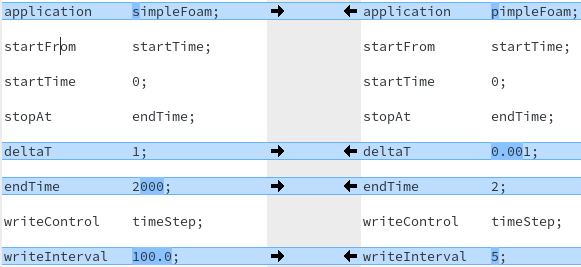
\includegraphics[width=0.8\textwidth]{Figuras/02_controlDict_1.png}}
	\caption{cambios en controlDict: caso estacionario (izquierda) vs caso transitorio (derecha)} \label{fg:controlDict}
\end{figure*}

\textbf{Nota: } Las cambios representados en las imágenes de este informe pueden diferir de las modificaciones finales reales. La última versión de cada archivo puede verse en el repositorio online.

En el archivo \href{https://github.com/guillerolle/casos_cfd/tree/master/04/case/system/fvSchemes}{fvSchemes} modificamos el campo \texttt{ddtSchemes} y agregamos una línea a \texttt{gradSchemes}. Los cambios se muestran en la figura \ref{fg:fvSchemes}.

\begin{figure*}[htb]
	\centerline{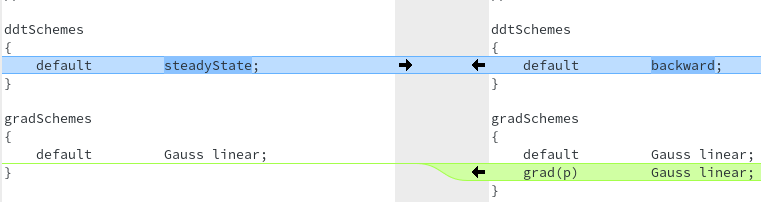
\includegraphics[width=0.8\textwidth]{Figuras/02_fvSchemes_1.png}} 
	\caption{cambios en fvSchemes: caso estacionario (izquierda) vs caso transitorio (derecha)} \label{fg:fvSchemes}
\end{figure*}

\newpage

Por último, modificamos las tolerancias de los solvers para \texttt{p} y \texttt{U} en el archivo \href{https://github.com/guillerolle/casos_cfd/tree/master/04/case/system/fvSolution}{fvSolution}. Además, agregamos los modificadores para el campo \texttt{PIMPLE}. los cambios se muestran en la figura \ref{fg:fvSolution}

\begin{figure*}[htb]
	\centerline{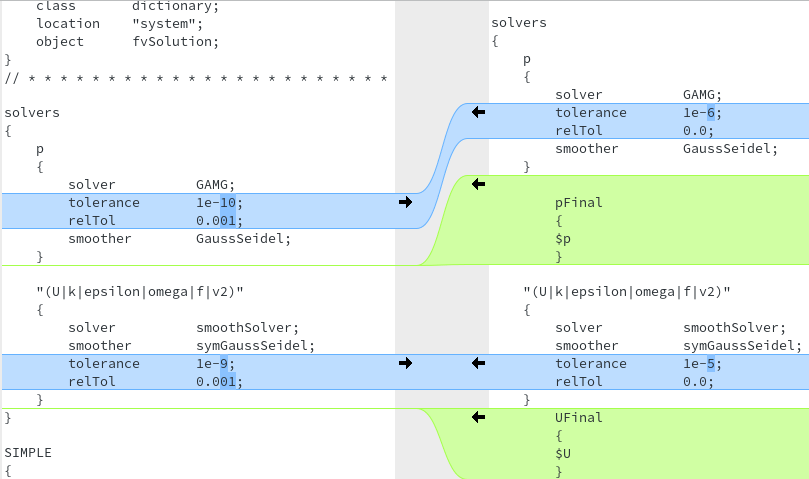
\includegraphics[width=0.8\textwidth]{Figuras/02_fvSolution_1.png}} 
	\centerline{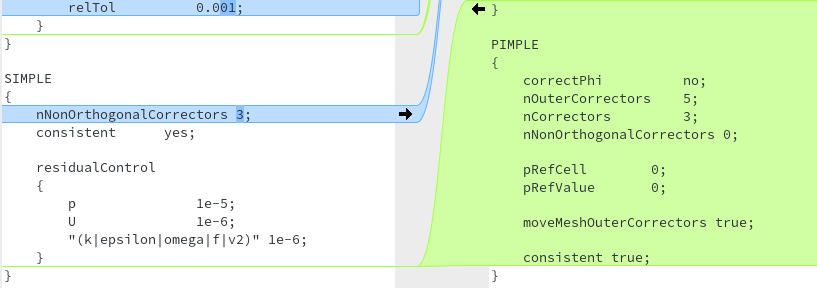
\includegraphics[width=0.8\textwidth]{Figuras/02_fvSolution_2.png}}
	\caption{cambios en fvSolution: caso estacionario (izquierda) vs caso transitorio (derecha)} \label{fg:fvSolution}
\end{figure*}


\newpage
\section{SIMULACIÓN}
Antes de poder ejecutar el archivo \href{https://github.com/guillerolle/casos_cfd/tree/master/04/case/Allrun}{Allrun} debemos modificarlo para que ejecute el solver \texttt{pimpleFoam} (ver figura \ref{fg:Allrun}). Además, recordar que en cada computadora donde se desee ejecutar este caso, se debe modificar el campo \texttt{FOAMDIR} del mismo archivo, y la cantidad de procesadores a utilizar con \texttt{mpirun}. Este último cambio debe corresponderse con el valor del campo \texttt{numberOfSubdomains} en el archivo \href{https://github.com/guillerolle/casos_cfd/tree/master/04/case/system/decomposeParDict}{decomposeParDict}.

\begin{figure*}[htb]
	\centerline{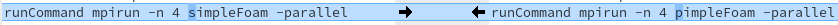
\includegraphics[width=1\textwidth]{Figuras/03_Allrun.png}} 
	\caption{cambios en Allrun: caso estacionario (izquierda) vs caso transitorio (derecha)} \label{fg:Allrun}
\end{figure*}

Con esto estamos listos para ejecutar la simulación:\\
\texttt{\$ ./Allrun}

Es posible que la simulación se ejecute durante un tiempo prolongado. Por suerte, podemos observar el caso en \textit{ParaView} mientras aún se está ejecutando como se ve en la figura \ref{fg:pv_time}. Para esto, en otra terminal ir al directorio del caso y ejecutar:\\
\texttt{\$ paraFoam -builtin}

\begin{figure*}[htb]
	\centerline{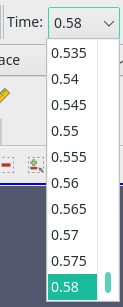
\includegraphics[width=0.2\textwidth]{Figuras/03_PV_TiempoIncompleto.png}} 
	\caption{Lista de tiempos incompleta en ParaView. El tiempo total de simulación es 2} \label{fg:pv_time}
\end{figure*}

Seleccionamos las opciones \textit{"Decomposed Case"} y \textit{"Skip Zero Time"} y podremos trabajar con los datos cargados actualmente. Al hacer click en \textit{"Refresh"} podremos cargar los nuevos pasos de tiempo que hayan sido guardados en el disco.

\begin{figure*}[htb]
	\centerline{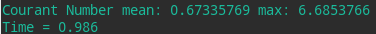
\includegraphics[width=0.6\textwidth]{Figuras/03_Courant.png}} 
	\caption{Valor medio y máximo del número de Courant para una iteración arbitraria} \label{fg:Courant}
\end{figure*}

Mientras se ejecuta el caso es importante observar los valores del \href{https://www.openfoam.com/documentation/guides/latest/doc/guide-fos-field-courant-no.html}{número de Courant}. Este número representa una medida de la velocidad con la que la información es transportada bajo la influencia de un campo de flujo. Es un factor limitante en el rendimiento de los esquemas numéricos. Es recomendable que este número no sea superior a que 1. En la figura \ref{fg:Courant}  se ve que el valor máximo de Courant para ese tiempo es muy alto (6.69). Esto lo podemos comprobar en la figura \ref{fg:pvCourant}. En la imagen, la escala está limitada a un valor máximo de 1. Hay una cantidad importante de celdas donde el valor de Courant es muy alto.

\begin{figure*}[htb]	
	\centerline{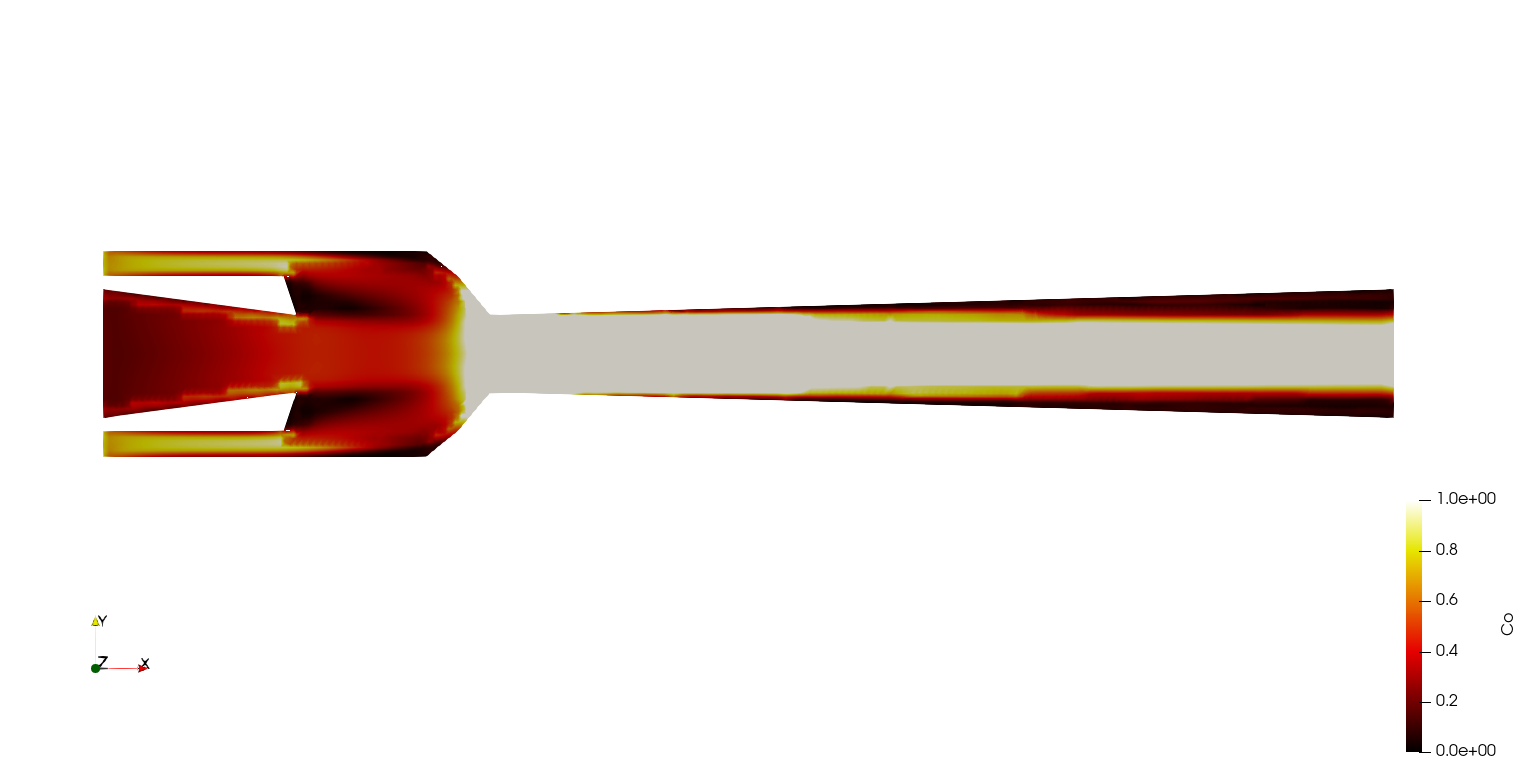
\includegraphics[width=1\textwidth]{Figuras/03_pvCourant1.png}} 
	\caption{Valor medio y máximo del número de Courant para una iteración arbitraria con h=0.001s} \label{fg:pvCourant}
\end{figure*}

Es posible que la simulación sea aceptable incluso para estos valores del número de Courant, pero para mejorar los resultados de la simulación, se cancela la simulación actual (\texttt{Ctrl+C} en la terminal) y se simula nuevamente con un paso de tiempo 10 veces más chico. Se espera que el número de Courant varíe linealmente con el paso de tiempo por su definición. Esta simulación es considerablemente más lenta (tardó aproximadamente 6 horas).

\begin{figure*}[htb]
	\centerline{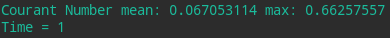
\includegraphics[width=0.6\textwidth]{Figuras/03_Courant2.png}} 
	\caption{Valor medio y máximo del número de Courant para una iteración arbitraria con h=0.0001s} \label{fg:Courant2}
\end{figure*}

En las figuras \ref{fg:Courant2} y \ref{fg:pvCourant2} se observa la clara disminución del número de Courant. Como mencionamos en el párrafo anterior, los valores medios y máximos (así como en todo el campo de flujo) se redujo aproximadamente 10 veces estos valores.

\begin{figure*}[htb]
	\centerline{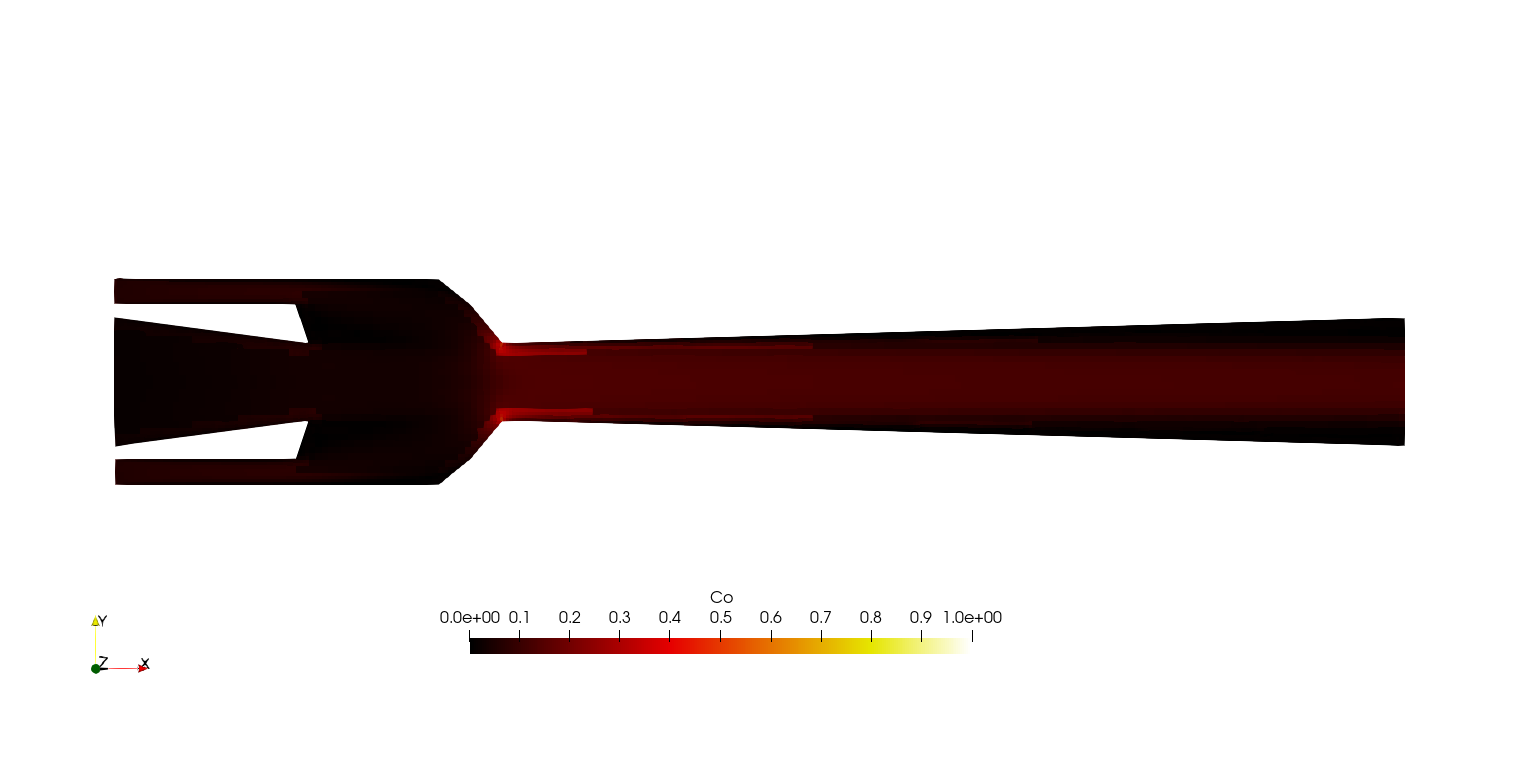
\includegraphics[width=1\textwidth]{Figuras/03_pvCourant2.png}} 
	\caption{Valor medio y máximo del número de Courant para una iteración arbitraria con h=0.0001s} \label{fg:pvCourant2}
\end{figure*}

\section{TIEMPO TRANSITORIO}
Con esta simulación podemos determinar el tiempo que demora el dispositivo en llegar al régimen estacionario. El solver \textit{pimpleFoam} deja de iterar cuando se satisfacen las tolerancias definidas en el archivo \texttt{fvSolution}. Podemos aprovechar el archivo \texttt{log} generado para determinar cuándo llegó a la solución estacionaria.

\texttt{\$ foamLog log.pimpleFoam}
En la carpeta \texttt{\$CASE\_DIR/logs} se encuentran todos los archivos de post-proceso producidos por el comando anterior. En la figura \ref{fg:iter0} se observa que para un tiempo aproximadamente mayor a 0.6 podemos asumir que el solver ya ha convergido lo suficiente a la solución estacionaria. 

\begin{figure*}[htb]
	\centerline{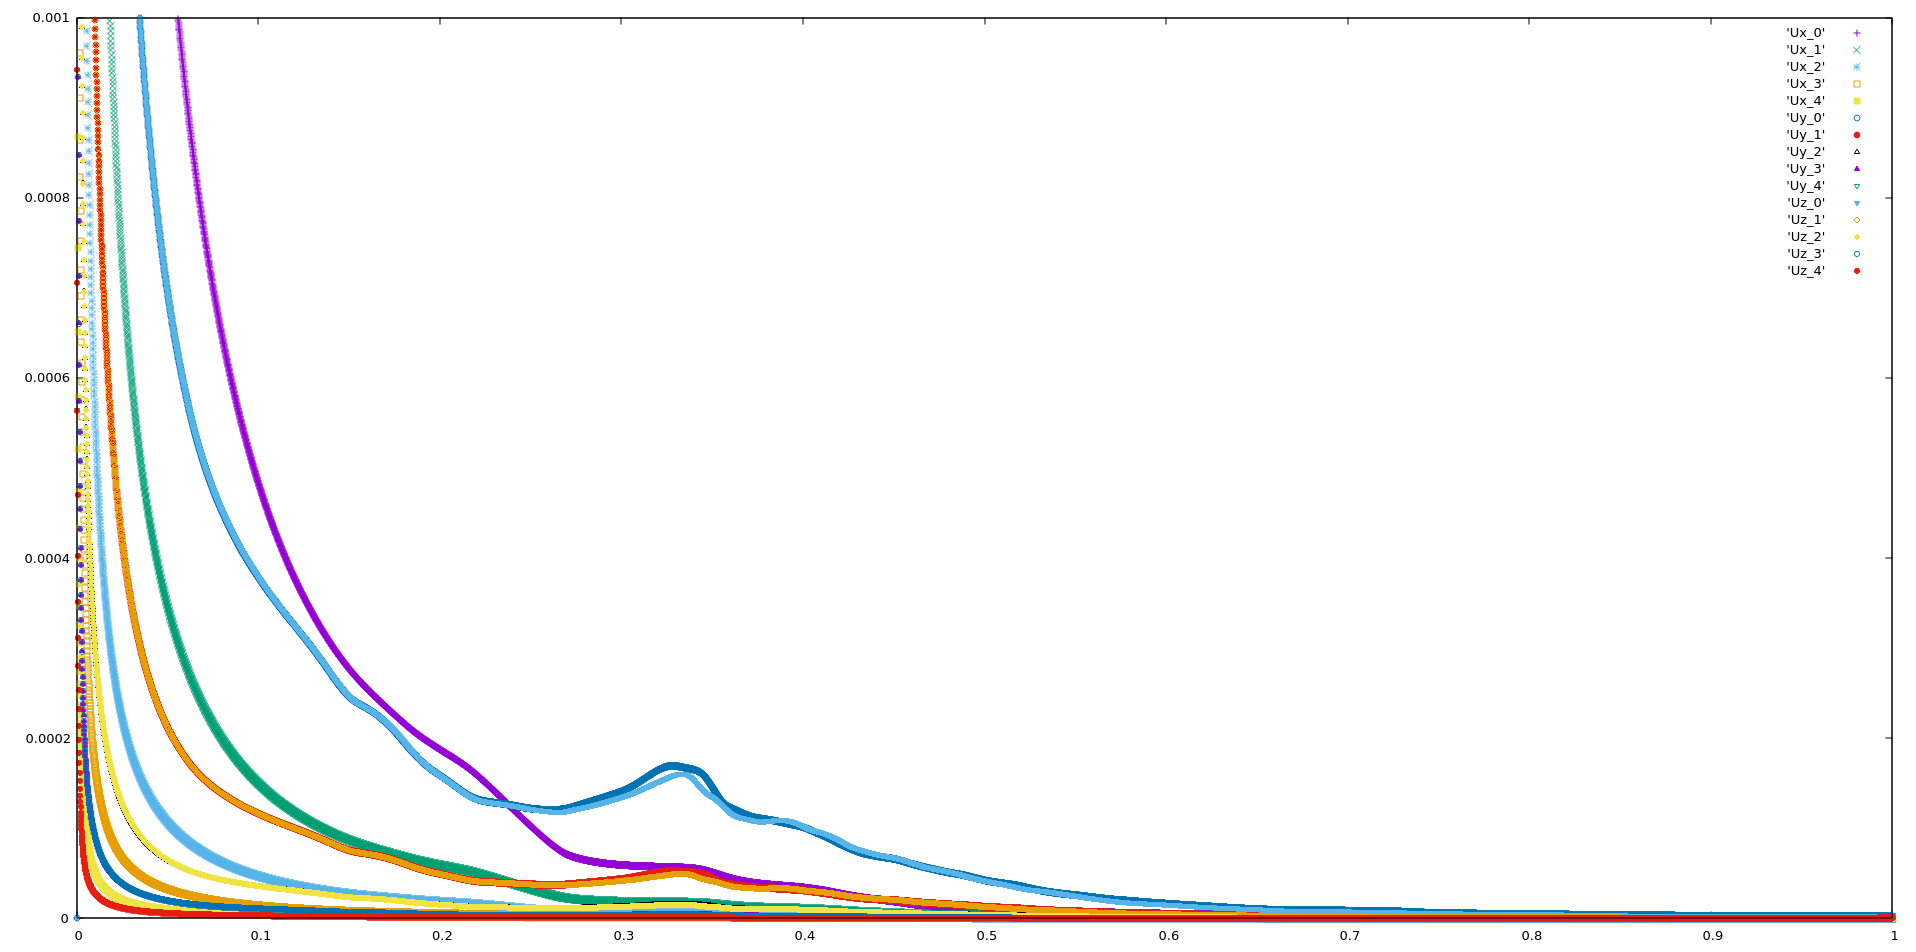
\includegraphics[width=0.8\textwidth]{Figuras/04_iter.png}} 
	\caption{Variaciones en U en cada iteración del método} \label{fg:iter0}
\end{figure*}

En la figura \ref{fg:05_compara_cte} se compara la simulación en tres tiempos diferentes para observar esas mínimas diferencias en el campo de velocidad (imperceptibles).

\begin{figure*}[htb]
	\centerline{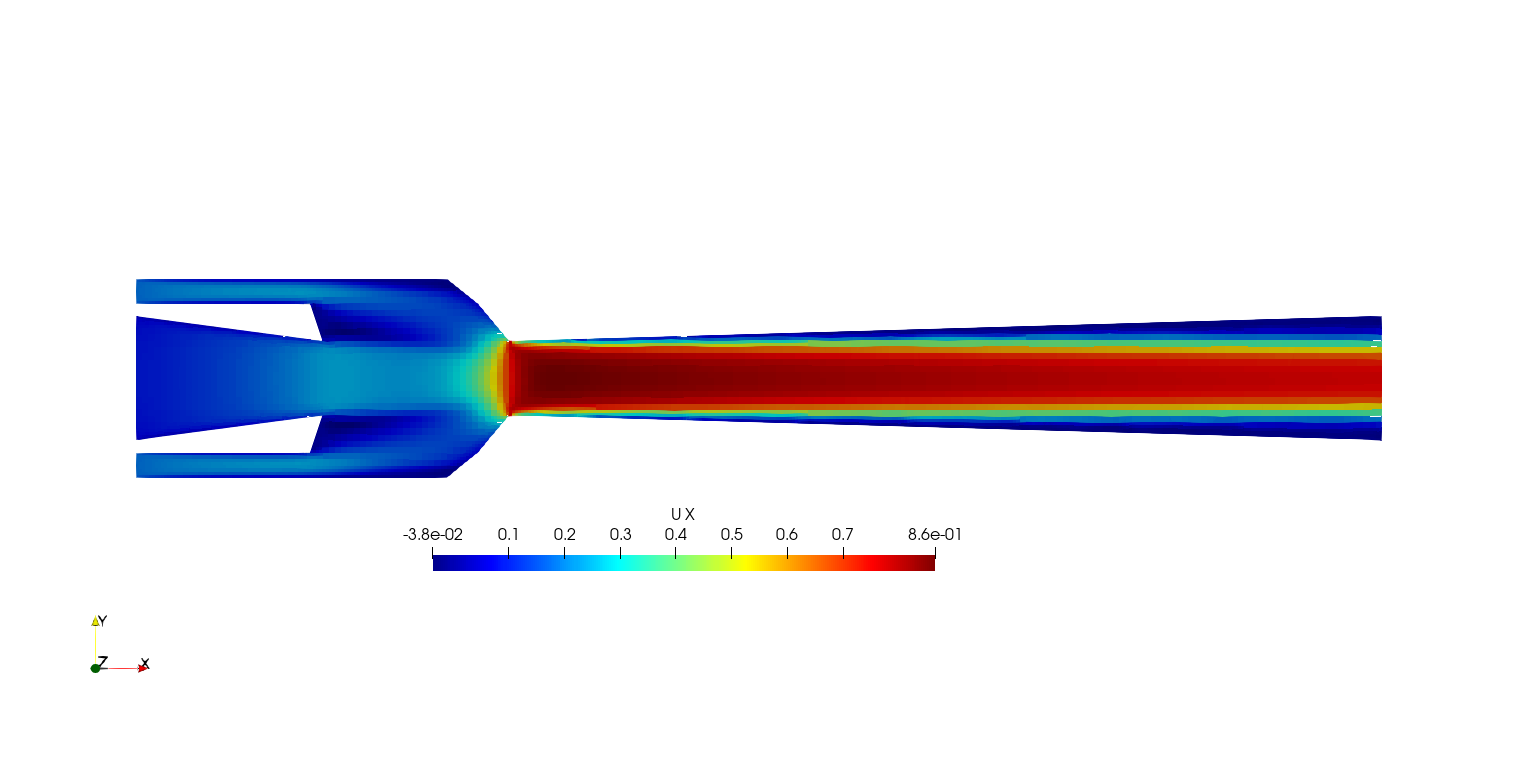
\includegraphics[width=0.8\textwidth]{Figuras/05_Ux_06.png}} 
	\centerline{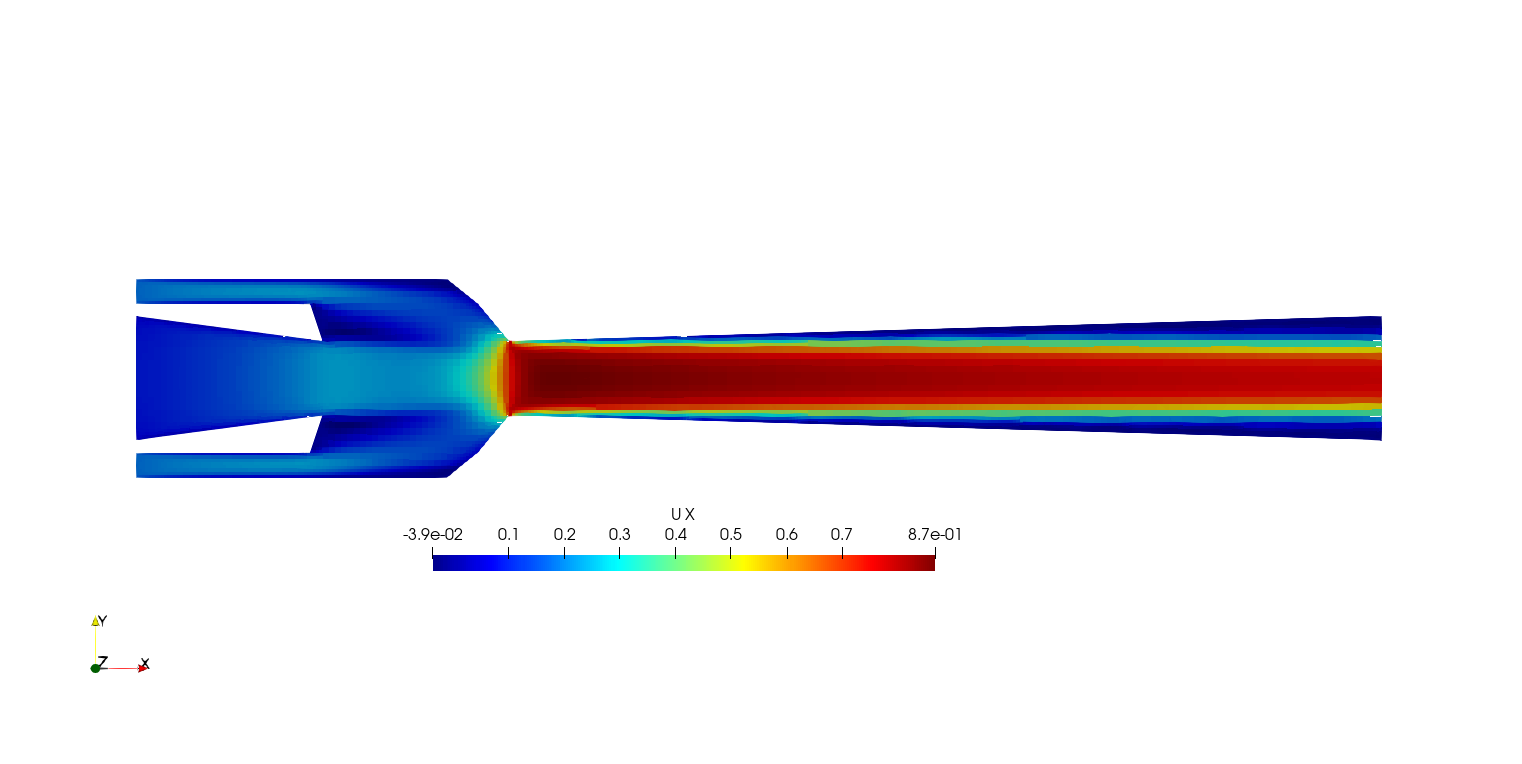
\includegraphics[width=0.8\textwidth]{Figuras/05_Ux_08.png}} 
	\caption{Campo Ux para t=0.6 (arriba) y t=0.8 (abajo)} \label{fg:05_compara_cte}
\end{figure*}

%\newpage
\section{COMPARACIÓN ENTRE SOLVERS}
Otro aspecto interesante es verificar si las simulaciones \texttt{simpleFoam} y \texttt{pimpleFoam} convergen a la misma solución estacionaria (o lo suficientemente parecidas). En la figura \ref{fg:06_pimple_simple} se comparan las dos simulaciones. Los resultados visibles son idénticos. También se comparan los campos de presión en la figura \ref{fg:06_pimple_simple_p}.

\begin{figure*}[htb]
	\centerline{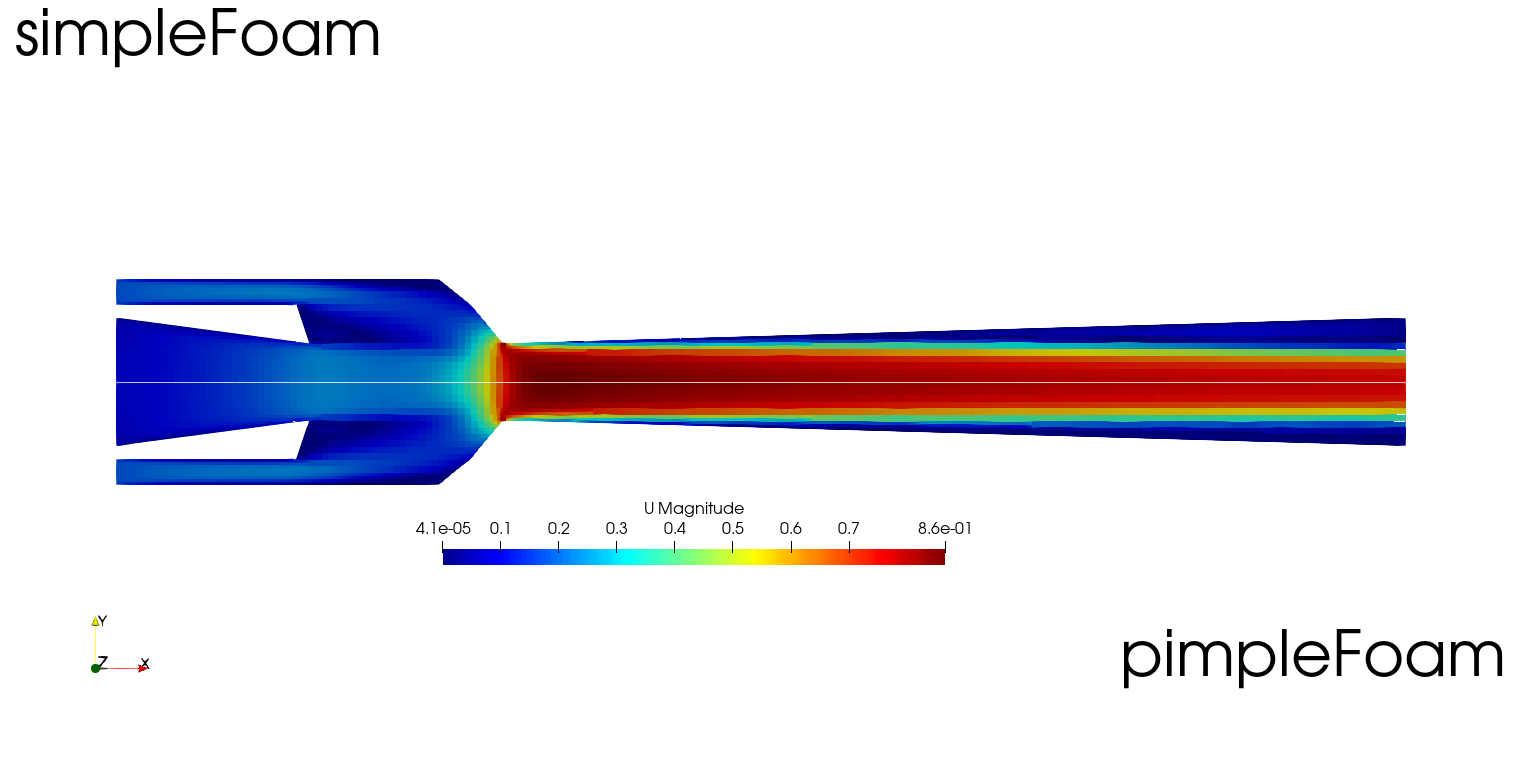
\includegraphics[width=0.8\textwidth]{Figuras/06_pimple_simple.png}} 
	\caption{Comparación campo U entre ambos solvers} \label{fg:06_pimple_simple}
\end{figure*}

\newpage
\begin{figure*}[htb]
	\centerline{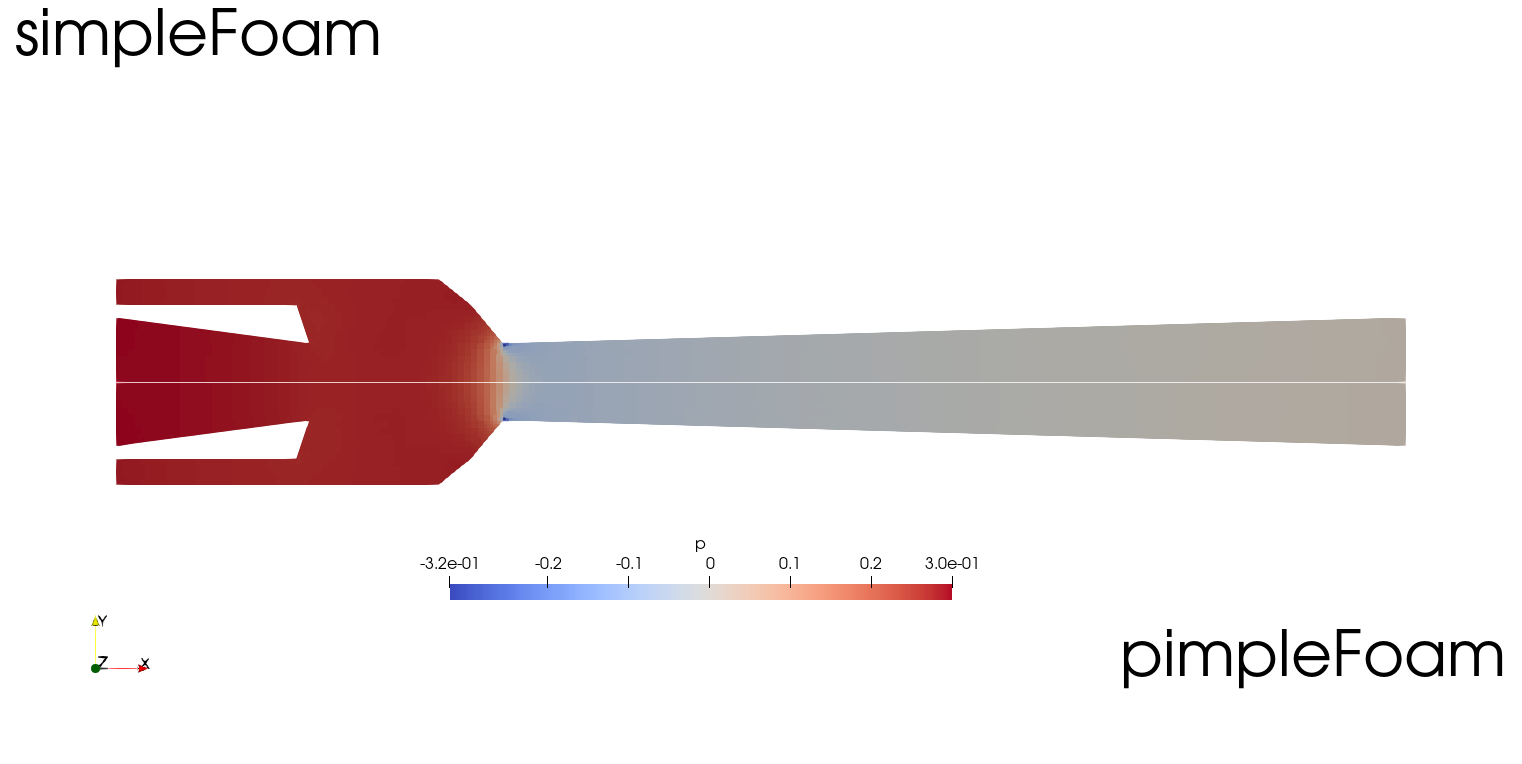
\includegraphics[width=0.8\textwidth]{Figuras/06_pimple_simple_p.png}} 
	\caption{Comparación campo P entre ambos solvers} \label{fg:06_pimple_simple_p}
\end{figure*}

Por último, vamos a comparar las diferencias en los campos en las primeras iteraciones de cada uno de los solvers.
Esto se ve en la figura \ref{fg:06_ps_transitorio} . Observar que el \textit{simpleFoam} con 100 iteraciones ya prácticamente ha convergido a la solución final. En un solver transitorio, la simulación varía con el número de iteración según el paso de tiempo. En la figura \ref{fg:06_ps_transitorio} se visualiza la iteración 500 de \textit{pimpleFoam}, es decir, el tiempo 0.05 s y se nota claramente que el flujo no está desarrollado y los transitorios no son comparables entre solvers.

\newpage
\begin{figure*}[htb]
	\centerline{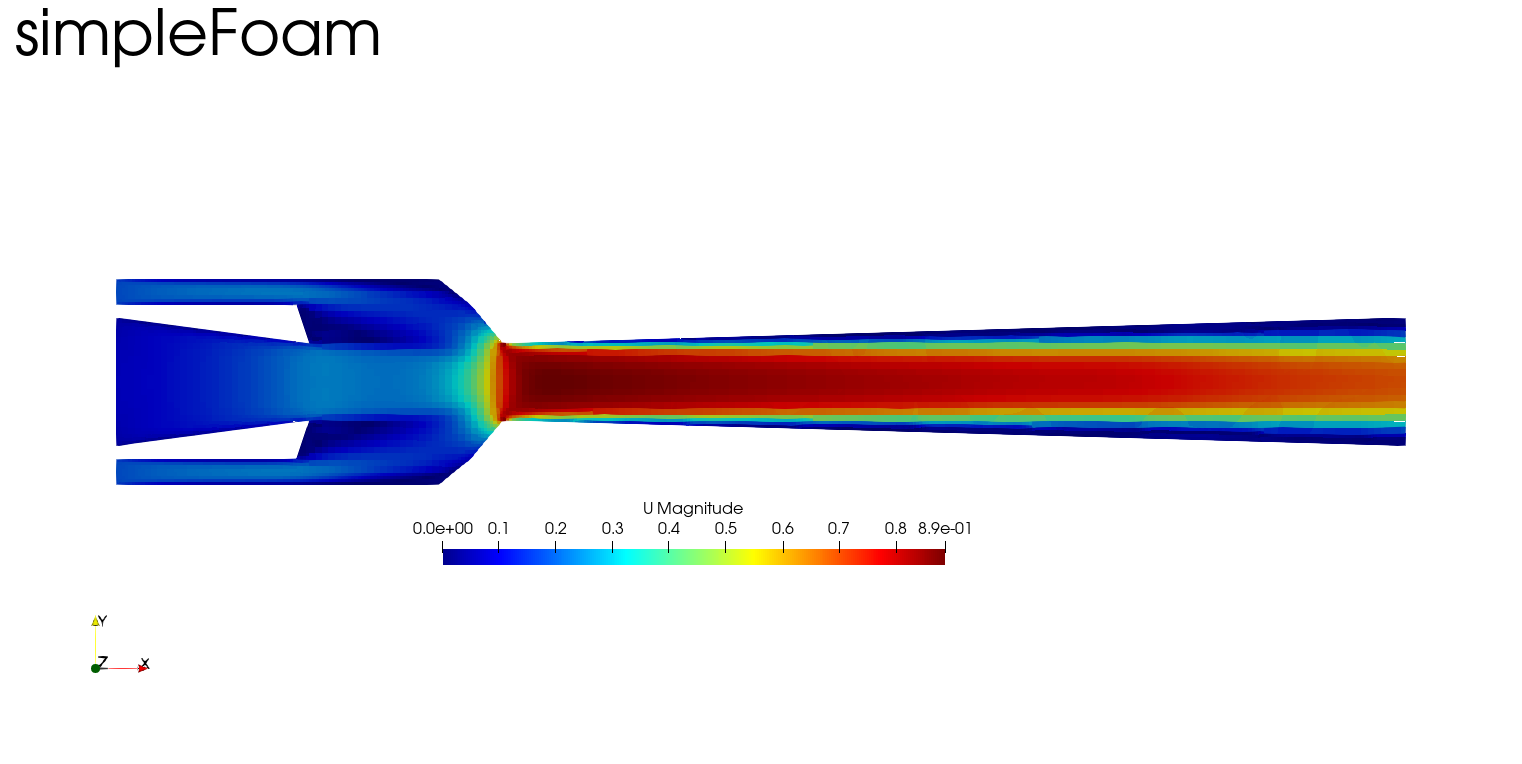
\includegraphics[width=0.8\textwidth]{Figuras/06_simple_100.png}} 
	\centerline{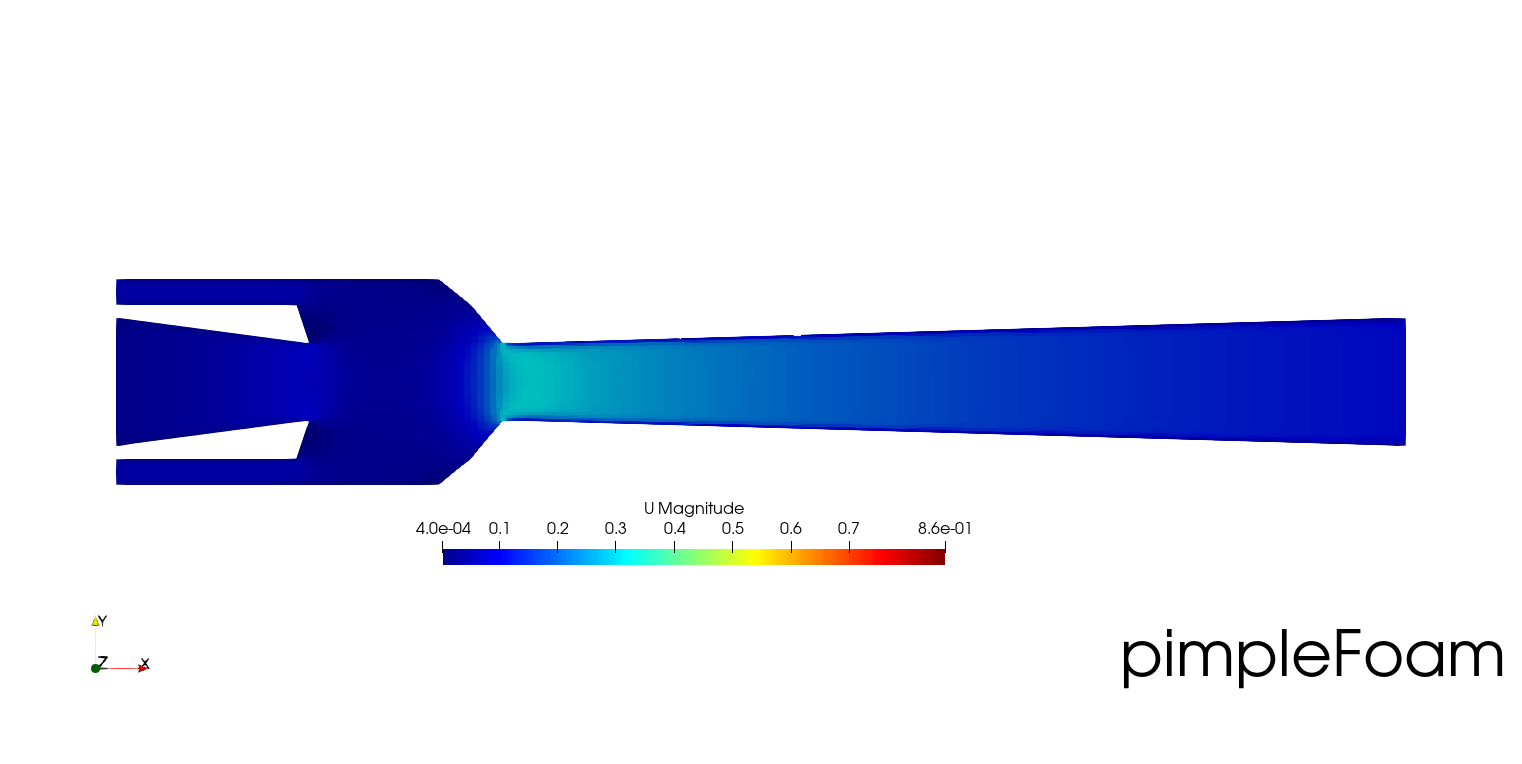
\includegraphics[width=0.8\textwidth]{Figuras/06_pimple_005.png}} 
	\caption{It. 100 de simpleFoam (arriba), It. 500 de pimpleFoam (abajo)} \label{fg:06_ps_transitorio}
\end{figure*}


\section{CONCLUSIONES}
En este informe ejecutamos la primera simulación transitoria con \textit{pimpleFoam} sobre un caso previo de \textit{simpleFoam}. Se analizaron algunas cuestiones propias de estos solvers como el \textit{Número de Courant} y el  tiempo de transitorio. También se verificó que los resultados del campo estacionario sean coherentes entre solvers.

En los informes anteriores se simulaba también la difusión y convección del agroquímico que es inyectado en el dispositivo. En este caso se omitió ese paso porque es el método utilizado es incompatible con este solver. Antes se obtenía el campo estacionario y luego, a partir de ese campo obtenido, se ejecutaba una simulación transitoria sobre la difusión del agroquímico (campo escalar). Como se utiliza un solver transitorio para calcular los campos de velocidad y presión en este informe, no es posible aplicar el mismo método.

El estudio de difusión de agroquímico en un campo transitorio se dejará para un informe futuro.

%\section*{AGRADECIMIENTOS} Los autores agradecen a ...
% ACKNOWLEDGEMENTS FOR FULL ARTICLES
%
%\bibliography{amcapaper}
\end{document}
